\documentclass[11pt]{article}
\usepackage[margin=1in]{geometry}
\usepackage{amsmath,amssymb,booktabs,graphicx,xcolor,hyperref}
\usepackage[most]{tcolorbox}
\hypersetup{colorlinks=true,linkcolor=blue!50!black,urlcolor=blue!50!black}
\newcommand{\dd}{\mathrm{d}}
\newcommand{\pX}{\partial_X}
\title{Analytic cosmological derivatives of the Limber $C_\ell^{ss}$ and $\xi_\pm$\\
\large Chain rule on Python-side response tables (plan for \texttt{cosmo2D\_fisher.c})}
\author{Cocoa / CosmoLike --- design note}
\date{2026-09-27 (C draft validated; cosmolike noise test)}

\begin{document}
\sloppy
\maketitle

\begin{tcolorbox}[colback=gray!6,colframe=gray!50,title=Summary]
Differentiating the Limber integral under the integral sign gives every
cosmological derivative of $C^{ij}_{ss}(\ell)$ --- and, by linearity, of
$\xi_\pm^{ij}(\theta)$ --- in closed form. The only inputs are four responses
per parameter $X$, supplied from Python on the same grids as
\texttt{set\_cosmology}:
\[
R_X(k,z)=\frac{\partial\ln P_{\rm NL}}{\partial X}\Big|_{k,z},\quad
\chi_X(z)=\frac{\partial\chi}{\partial X}\Big|_{z},\quad
\frac{\partial \ln G}{\partial X}\Big|_{z},\quad
\epsilon_X=\frac{\partial\ln\Omega_m}{\partial X}.
\]
Everything else --- $H(z)$ and its response, the lensing-efficiency
integral, the $k=\ell/\chi$ shift of $P_{\rm NL}$, the measure, the NLA
amplitude --- is analytic, using cubic-spline derivatives of $\chi(z)$ and
$\chi_X(z)$ and the bicubic-spline slope $\partial\ln P_{\rm NL}/\partial\ln k$.
\textbf{Verified} against central finite differences of the full $C_\ell$
for $\ln A_s$, $\Omega_m$ and $w_0$ (halofit, NLA): agreement
$\le 1.1\times10^{-4}$ at $30\le\ell\le3000$ (Table~\ref{tab:exact}), the
level of the finite-difference truncation itself. The $w_0$ case uses no
parameter-specific code.

\textbf{What cannot be avoided:} $R_X(k,z)$. It is not contained in any
single-cosmology $P(k,z)$ table; the best table-only models miss
$d\ln C/d\ln A_s$ by up to 35\% and $d\ln C/d\Omega_m$ by up to 27\%
(Sec.~\ref{sec:tableonly}). So the Python side must provide it (e.g.\
central differences of the CAMB tables only). \textbf{Scope:} NLA
intrinsic alignments; TATT is excluded (its one-loop kernels need the
FAST-PT FFTs of the response, which would complicate cosmolike).
\end{tcolorbox}

\section{The integral cosmolike computes}
In cosmolike units ($\chi$ in $c/H_0$, $k$ in $H_0/c$, both fixed in $h$-units),
the Limber shear--shear spectrum for source bins $i,j$ is an integral over the
scale factor between parameter-independent limits (the source $n(z)$ support is
fixed in redshift):
\begin{equation}
C^{ij}(\ell)=\Pi(\ell)\int_{a_{\min}}^{a_{\max}}\!\dd a\;
\underbrace{\frac{\chi'(a)}{\chi^2(a)}}_{w(a)}\;
q_i(a)\,q_j(a)\;P_{\rm NL}\!\big(k_\ell(a),z(a)\big),
\qquad k_\ell=\frac{\ell+\tfrac12}{\chi(a)},
\label{eq:cl}
\end{equation}
with $\chi'(a)\equiv|\dd\chi/\dd a|=\chi_z/a^2$ (cosmolike's \texttt{dchida}) and
$\Pi(\ell)=(\ell-1)\ell(\ell+1)(\ell+2)/(\ell+\tfrac12)^4$ (1812.05995 eqs.~74--79).
For NLA the E-mode kernel factorizes per bin ($C_{BB}=0$):
\begin{align}
q_b &= W_{\kappa,b}-W_{s,b}\,C_1, &
W_{\kappa,b}&=\tfrac32\,\Omega_m\,\frac{\chi}{a}\,g_b(a), &
W_{s,b}&=n_b(z)\,E(z),\\
g_b(a)&=\mathcal P_b(a)-\chi(a)\,\mathcal Q_b(a), &
\mathcal P_b&=\!\int_{a_{\min}}^{a}\!\!\frac{\dd a'}{a'^2}\,n_b, &
\mathcal Q_b&=\!\int_{a_{\min}}^{a}\!\!\frac{\dd a'}{a'^2}\,\frac{n_b}{\chi(a')},
\end{align}
$E(z)=H/H_0=1/\chi_z(z)$ with $\chi_z\equiv\dd\chi/\dd z$ (the cosmolike
\texttt{hoverh0}), and the NLA amplitude
$C_1(z)=A(z)\,\Omega_m\,\bar C_1\rho_{\rm cr}/D(z)$, $D(0)=1$.

\section{Differentiating under the integral}
Because $a$ and the limits in Eq.~\eqref{eq:cl} do not depend on the
cosmology, $\partial_X$ commutes with the integral. Differentiate at fixed $a$
(equivalently fixed $z$):
\begin{equation}
\boxed{\;
\pX C^{ij}(\ell)=\Pi(\ell)\!\int\!\dd a\;w\,P_{\rm NL}
\Big[\Lambda_X(\ell,a)\,q_iq_j+(\pX q_i)\,q_j+q_i\,(\pX q_j)\Big]\;}
\label{eq:master}
\end{equation}
with $\Lambda_X=\pX\ln w+\pX\ln P_{\rm NL}$. Every factor follows from the
four inputs:

\paragraph{Measure.} $w=\chi'/\chi^2$ and $\chi'=\chi_z/a^2$ at fixed $a$, so
\begin{equation}
\pX\ln w=\frac{\chi_X'(z)}{\chi_z(z)}-2\,\frac{\chi_X}{\chi},
\end{equation}
where $\chi_X'\equiv\dd\chi_X/\dd z$ is the \emph{cubic-spline derivative}
of the input $\chi_X(z)$.

\paragraph{Power spectrum.} $P_{\rm NL}$ depends on $X$ explicitly and through
$k_\ell=\ell/\chi$:
\begin{equation}
\pX\ln P_{\rm NL}\big(k_\ell(a),z\big)=
-\,n_{\rm eff}(k_\ell,z)\,\frac{\chi_X}{\chi}+R_X(k_\ell,z),
\qquad n_{\rm eff}\equiv\frac{\partial\ln P_{\rm NL}}{\partial\ln k}
\end{equation}
($n_{\rm eff}$ from the bicubic spline of $\ln P_{\rm NL}$). The first term is
the chain rule the spline provides; the second is the explicit response,
which no spline of one table can provide (Sec.~\ref{sec:tableonly}).

\paragraph{Expansion rate.} $E=1/\chi_z$ gives $\pX\ln E=-\chi_X'/\chi_z$ ---
again only the spline derivative of $\chi_X$.

\paragraph{Lensing efficiency.} $\mathcal P_b$ is cosmology-independent;
$\pX\mathcal Q_b=-\int\dd a'\,a'^{-2}n_b\,\chi_X/\chi^2$. Hence
\begin{equation}
\pX g_b=-\chi_X\,\mathcal Q_b+\chi\,\mathcal R_b,\qquad
\mathcal R_b(a)=\int_{a_{\min}}^{a}\frac{\dd a'}{a'^2}\,
\frac{n_b(z')\,\chi_X(a')}{\chi^2(a')},
\end{equation}
one more cumulative trapezoid on the same fine grid \texttt{g\_tomo} uses.

\paragraph{Kernels.}
\begin{align}
\pX W_{\kappa,b}&=W_{\kappa,b}\Big(\epsilon_X+\frac{\chi_X}{\chi}\Big)
+\tfrac32\Omega_m\frac{\chi}{a}\,\pX g_b,\\
\pX W_{s,b}&=-W_{s,b}\,\frac{\chi_X'}{\chi_z},\\
\pX C_1&=C_1\big(\epsilon_X-\gamma_X\big),\qquad
\gamma_X(z)=\frac{\partial\ln G}{\partial X}(z)-\frac{\partial\ln G}{\partial X}(0),
\end{align}
the last because cosmolike's $D(z)=a\,G(z)/G(0)$ is normalized at $z=0$.
Then $\pX q_b=\pX W_{\kappa,b}-(\pX W_{s,b})C_1-W_{s,b}\,\pX C_1$.

\paragraph{Structure.} Per quadrature node, $w P$, $\Lambda_X$, $q_b$ and
$\pX q_b$ are precomputed; the $(\ell,{\rm pair})$ fill of
Eq.~\eqref{eq:master} is then the same branch-free SIMD reduction as
\texttt{C\_ss\_tomo\_limber\_work}, computing $C^{ij}$ and all $\pX C^{ij}$ in
one pass.

\section{Real space}
cosmolike's $\xi_\pm^{ij}(\theta)=\sum_\ell G_\pm(\ell,\theta)\,
[C^{ij}_{EE}(\ell)\pm C^{ij}_{BB}(\ell)]$ uses bin-averaged Legendre kernels
$G_\pm$ that do not depend on the cosmology, so the map is linear and exact:
\begin{equation}
\pX\xi_\pm^{ij}(\theta)=\sum_\ell G_\pm(\ell,\theta)\,\pX C^{ij}_{EE}(\ell),
\qquad
\pX\ln\xi_\pm=\pX\xi_\pm/\xi_\pm .
\end{equation}
In practice $\pX C$ is tabulated on the log-$\ell$ grid and gathered to every
integer $\ell$ with \texttt{limber\_fill\_interp}, exactly as \texttt{xi\_pm\_tomo}
does for $C$. Shear calibration $(1+m_i)(1+m_j)$ multiplies outside and
cancels in $\pX\ln\xi_\pm$.

\section{Verification}
A Python implementation of Eqs.~(\ref{eq:cl})--(\ref{eq:master}) (CAMB,
Takahashi halofit, $m_\nu=0.06$\,eV, two Gaussian source bins at $z=0.5,1.1$,
NLA with $A_1=0.6$, $\eta=-1.5$) takes the four inputs as central
differences of the CAMB tables on fixed grids --- exactly what the Python side
would hand to cosmolike. The truth is the central difference of the full
$C_\ell$, recomputing geometry, kernels, growth and $P_{\rm NL}$ at $X\pm h$
($h=0.01$ in $\ln A_s$, $0.005$ in $\Omega_m$, $0.02$ in $w_0$).

\begin{table}[h]
\centering\small
\caption{$\dd\ln C^{ij}/\dd X$: finite difference, and analytic/FD$-1$.}
\label{tab:exact}
\begin{tabular}{rc|rr|rr|rr}
\toprule
& & \multicolumn{2}{c|}{$X=\ln A_s$} & \multicolumn{2}{c|}{$X=\Omega_m$}
& \multicolumn{2}{c}{$X=w_0$}\\
$\ell$ & bins & FD & rel.\ diff & FD & rel.\ diff & FD & rel.\ diff\\
\midrule
30 & (0,0) & 1.02396 & -2.4e-06 & 8.16100 & -5.2e-05 & -0.85127 & -1.0e-05 \\
30 & (1,1) & 1.00113 & -5.2e-07 & 5.87218 & -5.1e-05 & -0.79806 & -2.4e-05 \\
30 & (0,1) & 1.01284 & -1.4e-06 & 7.40933 & -5.3e-05 & -0.86004 & -1.7e-05 \\
100 & (0,0) & 1.19447 & +9.5e-06 & 10.70446 & -2.1e-05 & -0.94115 & -4.8e-05 \\
100 & (1,1) & 1.06280 & +6.6e-06 & 8.40663 & -4.1e-05 & -0.89853 & -5.0e-05 \\
100 & (0,1) & 1.14412 & +9.4e-06 & 9.95070 & -2.5e-05 & -0.96658 & -6.2e-05 \\
300 & (0,0) & 1.45336 & -2.3e-05 & 12.19212 & -3.6e-05 & -0.96586 & -5.3e-05 \\
300 & (1,1) & 1.27960 & +3.3e-06 & 10.61055 & -3.2e-05 & -0.97054 & -8.9e-05 \\
300 & (0,1) & 1.41760 & -1.8e-05 & 11.75446 & -3.2e-05 & -1.00069 & -1.0e-04 \\
1000 & (0,0) & 1.42906 & -5.4e-05 & 12.15561 & -7.3e-05 & -0.92036 & +6.9e-05 \\
1000 & (1,1) & 1.48458 & -4.3e-05 & 11.92446 & -5.0e-05 & -0.97633 & -4.5e-05 \\
1000 & (0,1) & 1.47246 & -5.6e-05 & 12.13367 & -6.9e-05 & -0.97216 & -8.9e-06 \\
3000 & (0,0) & 1.14133 & -4.0e-05 & 10.75940 & -7.4e-05 & -0.77947 & +9.9e-05 \\
3000 & (1,1) & 1.32769 & -5.7e-05 & 11.48836 & -5.4e-05 & -0.88695 & -3.7e-05 \\
3000 & (0,1) & 1.19839 & -3.8e-05 & 10.90386 & -6.2e-05 & -0.85035 & +1.9e-05 \\

\bottomrule
\end{tabular}
\end{table}

\begin{figure}[h]
\centering
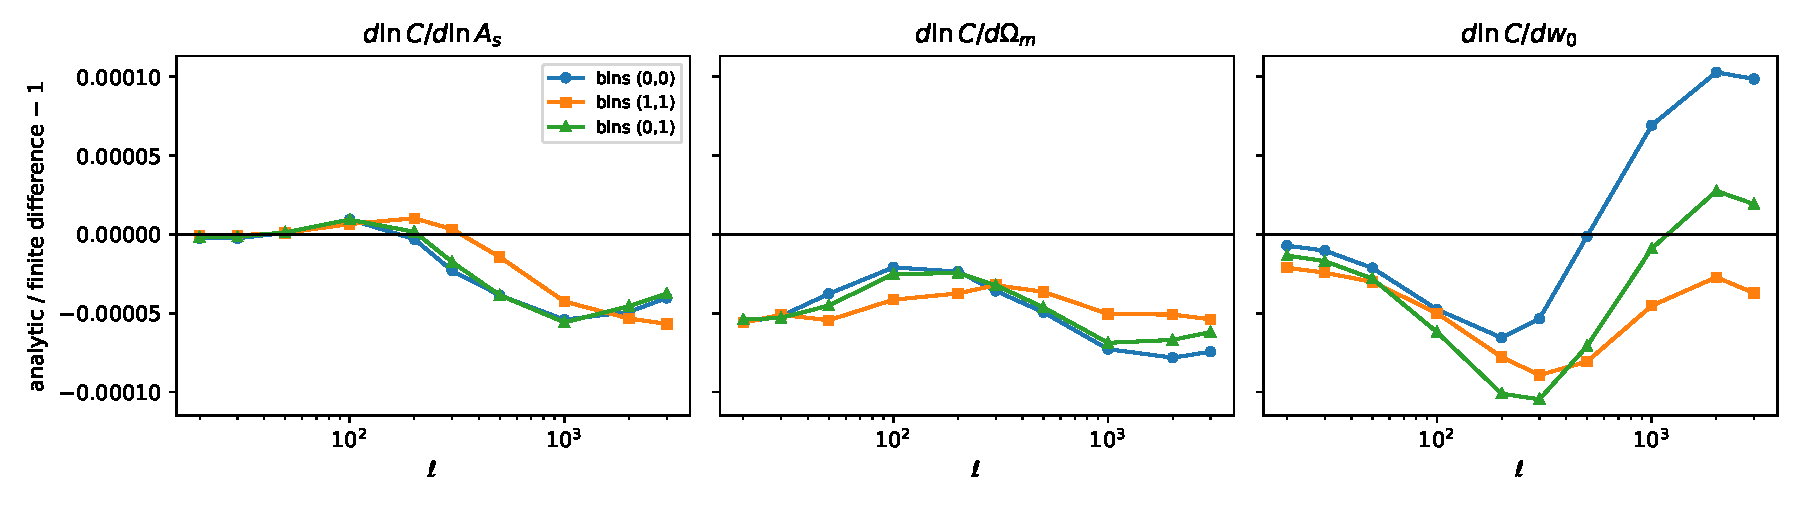
\includegraphics[width=\linewidth]{fisher_proto_exact.pdf}
\caption{Analytic derivative over finite difference, minus one. The residual
($\lesssim10^{-4}$) is the $O(h^2)$ truncation of the finite differences.}
\end{figure}

\section{Why $R_X$ must be an input}\label{sec:tableonly}
For $\ln A_s$ the projection terms vanish identically ($A_s$ does not touch
geometry, kernels or growth normalization), so the entire derivative is the
kernel-weighted average of $R_{A_s}$. We tested the two best ways to build
$R_X$ from the fiducial tables alone:
\begin{itemize}
\item \emph{Amplitude--redshift degeneracy:}
$R_{A_s}\approx\partial_z\ln P_{\rm NL}/\partial_z\ln P_{\rm L}$. Exact in
linear theory, but halofit depends on redshift also through $\Omega_m(z)$
(e.g.\ the one-halo slope $y^{3f_1(\Omega_m(z))}$), which contaminates the
$z$-derivative by $\sim0.3$ in $R$ at $k\gtrsim1\,h$/Mpc.
\item \emph{Shape shift for $\Omega_m$:} $\Gamma=\Omega_m h$ scaling of the
transfer function, amplitude via the degeneracy, growth from the
sensitivity ODE.
\end{itemize}

\begin{table}[h]
\centering\small
\caption{Table-only response models versus finite differences (bins $(0,0)$).}
\begin{tabular}{r|rrr|rrr}
\toprule
& \multicolumn{3}{c|}{$\dd\ln C/\dd\ln A_s$} & \multicolumn{3}{c}{$\dd\ln C/\dd\Omega_m$}\\
$\ell$ & FD & model & error & FD & model & error\\
\midrule
30 & 1.0240 & 1.0140 & -1.0\% & 8.1610 & 7.1515 & -12.4\% \\
100 & 1.1945 & 1.1764 & -1.5\% & 10.7045 & 9.1855 & -14.2\% \\
300 & 1.4534 & 1.4947 & +2.8\% & 12.1921 & 11.2529 & -7.7\% \\
1000 & 1.4291 & 1.6257 & +13.8\% & 12.1556 & 12.9572 & +6.6\% \\
3000 & 1.1413 & 1.5363 & +34.6\% & 10.7594 & 13.6514 & +26.9\% \\

\bottomrule
\end{tabular}
\end{table}

\begin{figure}[h]
\centering
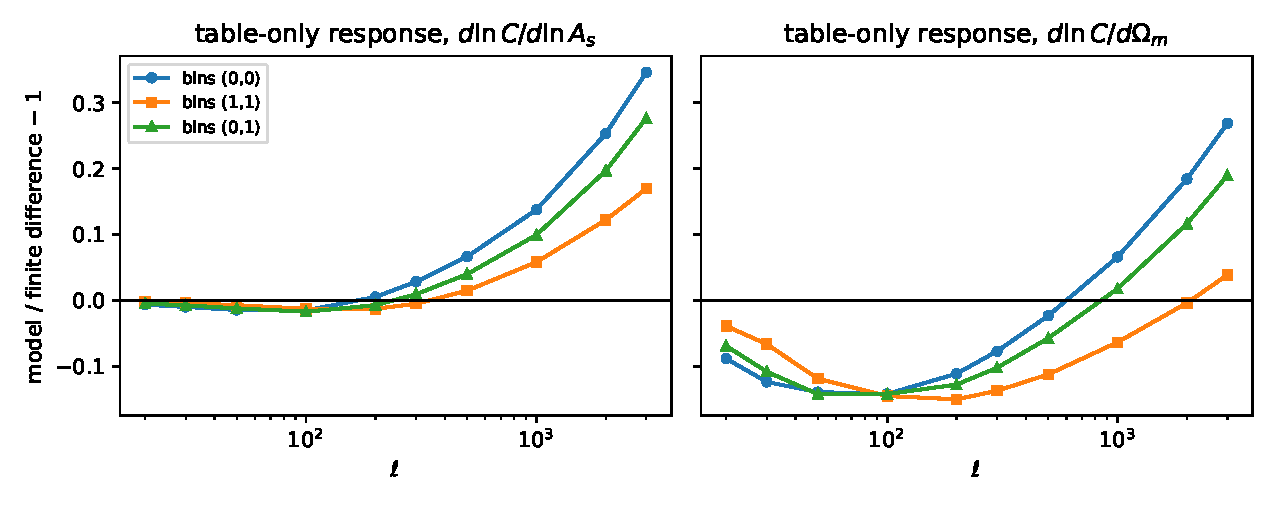
\includegraphics[width=0.8\linewidth]{fisher_proto_tableonly.pdf}
\caption{Table-only response models: errors of 10--35\% at $\ell\ge1000$.}
\end{figure}

\section{Cost and precision}
A finite-difference Fisher needs $2N$ (five-point: $4N$) CAMB runs
\emph{and} $2N$ ($4N$) full cosmolike evaluations. The analytic route needs
the same CAMB runs (to build $R_X$, $\chi_X$, $\partial_X\ln G$) but only
\emph{one} cosmolike pass that returns $C$ and all $N$ derivatives together.
Since CAMB dominates the wall time, the speed-up is on the cosmolike side
(the C draft returns $C$ plus three derivatives in $\sim$40\,ms, $\xi_\pm$
plus three derivatives in $\sim$90\,ms). On precision, the measurements of
Sec.~\ref{sec:draft} overturn the initial expectation that cosmolike's
interpolants make finite-difference Fishers noisy: cosmolike adds no
measurable noise, and the noise of the notebook Fisher is CAMB's halofit
(Sec.~\ref{sec:noise}), which a one-line CAMB fix removes. The analytic
route is therefore not needed for stability; it remains the natural
adapter for differentiable (JAX) Boltzmann codes, which give the four
inputs exactly by automatic differentiation.

\section{Validation of the C draft}\label{sec:draft}
\texttt{cosmo2d\_fisher.c} was built into a scratch copy of the lsst\_y1
interface (5 source bins, NLA) and checked two ways.

\paragraph{Chain rule, CAMB noise removed.} The perturbed cosmologies are
synthetic: every \texttt{set\_cosmology} table is the fiducial one moved
exactly along the loaded response
($\ln P_{\rm NL}\pm sR_X$, $\chi\pm s\chi_X$, $\ln G\pm s\,\partial_X\ln G$,
$\Omega_m(1\pm s\epsilon_X)$), and cosmolike's own $C_\ell$ and
\texttt{xi\_pm\_tomo} are differenced along that path. Maximum
$|{\rm analytic}/{\rm FD}-1|$ over $30\le\ell\le3000$ and all 15 pairs, at
$s=10^{-4}$: $4\times10^{-11}$ for $\ln A_s$, $5\times10^{-5}$ for
$\Omega_m$, $4\times10^{-4}$ for $w_0$ (step-independent: the analytic side
uses spline derivatives, cosmolike's $C$ piecewise-linear interpolants); for
$\xi_\pm$: $3\times10^{-9}$, $3\times10^{-6}$, $3\times10^{-5}$. The draft's
$C$ and $\xi_\pm$ themselves equal the likelihood's to $10^{-15}$ and
$5\times10^{-14}$.

\paragraph{Against real CAMB finite differences.} With the same step for
the response and for the finite difference, the two agree to
$\lesssim6\times10^{-4}$ for $\ell\le1000$. Both drift together with the
step (e.g.\ $d\ln C/d\ln A_s$ for bins $(4,4)$ at $\ell=1000$: 1.24, 1.50,
1.40, 1.44 at $s=0.0025$--$0.02$), and one-sided differences disagree by
up to $\sim$20\%: the fiducial CAMB table differs from the mean of the $\pm$
tables by up to $5\times10^{-3}$ in $\ln P_{\rm NL}$. That jitter, not
cosmolike, sets the precision floor.

\section{Does cosmolike add noise to finite-difference Fishers?}\label{sec:noise}
\paragraph{Cosmolike alone.} Along the smooth synthetic path above, finite
differences of cosmolike's $C_\ell$ and $\xi_+$ at Fisher-sized steps
converge to the analytic derivative as $s^2$ (3-point) and $s^4$ (5-point
stencil): for $\ln A_s$, $6.7\times10^{-13}$ at $s=10^{-3}$ and
$2.1\times10^{-6}$ at $s=0.06$ with the 5-point stencil. Pure truncation, no
noise.

\paragraph{CAMB.} $|\ln P(X_0)-\tfrac12[\ln P(X_0{+}s)+\ln P(X_0{-}s)]|$
reaches $5\times10^{-3}$ for $P_{\rm NL}$ (but $10^{-14}$ for $P_{\rm L}$) at
every CAMB accuracy setting tried (\texttt{AccuracyBoost} 1--3,
\texttt{CAMBAccuracyBoost} 2, \texttt{k\_per\_logint} 40). It is coherent
over whole redshift slices: CAMB's halofit stops the bisection for the
nonlinear scale at $|\sigma(R)-1|\le10^{-3}$
(\texttt{fortran/halofit.f90}, line~322), and the stopping point jumps with
the cosmology. Tightening the tolerance to $10^{-7}$ (a scratch CAMB build)
brings the jitter to $2.9\times10^{-5}$, the genuine curvature term, at no
measurable cost.

\paragraph{The notebook Fisher.} The lsst\_y1 notebook forecast (17
parameters, 5-point stencil, relative step $h$, FoM of $(A_s,\Omega_m)$)
reproduced at \texttt{AccuracyBoost}~1:
\begin{center}\small
\begin{tabular}{lrrrrr}
\toprule
case & $h=0.01$ & 0.02 & 0.03 & 0.05 & 0.08\\
\midrule
stock CAMB (the notebook) & 205.8 & 159.0 & 179.4 & 140.3 & 153.1\\
stock CAMB, CAMB boost 3 & 205.0 & 158.5 & 180.7 & 140.4 & 151.3\\
cosmolike only (synthetic inputs) & 152.71 & 152.71 & 152.71 & 152.72 & 152.80\\
halofit tolerance $10^{-7}$ & 146.0 & 145.8 & 145.6 & 145.6 & 147.1\\
\bottomrule
\end{tabular}
\end{center}
With the patched CAMB, \texttt{AccuracyBoost} 2 and 3 give 145.2 and 145.1
at $h=0.03$: once the jitter is gone, the finite-difference Fisher is
stable and converged at the default accuracy.

\section{Scope and caveats}
\begin{itemize}
\item \textbf{NLA only.} TATT one-loop kernels are FAST-PT convolutions of
$P_{\rm L}$; their response would need FFTs inside cosmolike. Excluded by
design; TATT Fisher stays on finite differences.
\item \textbf{Parameter-agnostic, with the explicit $\Omega_m$ in
$\epsilon_X$.} $\Omega_m$ appears explicitly twice --- the lensing prefactor
$\tfrac32\Omega_m(H_0/c)^2$ and the NLA amplitude
$\Omega_m\bar C_1\rho_{\rm cr}/D$ --- and both are carried by
$\epsilon_X=\partial\ln\Omega_m/\partial X$ at fixed other sampled
parameters. In Cocoa's basis ($\Omega_m,\Omega_b,H_0,A_s,n_s,m_\nu,w_0,w_a$):
$\epsilon_{\Omega_m}=1/\Omega_m$ and $\epsilon_X=0$ for all others --- for $h$
because $\Omega_m$ is itself sampled and cosmolike works in $h$-units (no
explicit $h$ in $(H_0/c)^2$ or $\bar C_1\rho_{\rm cr}$), for $m_\nu$ because
Cocoa's $\Omega_m$ includes the neutrinos. A basis sampling $\omega_m$
instead would give $\epsilon_h=-2/h$. With that one scalar per parameter,
the same code serves $A_s$, $\Omega_m$, $n_s$, $w_0$, $w_a$, $h$, $m_\nu$.
\item \textbf{$h$ and the $k$-grid.} The CAMB tables are shifted to
$h/$Mpc after evaluation, so for $X=h$ the perturbed tables must be
re-interpolated onto the fiducial grid before differencing; for every
other parameter the grids coincide.
\item \textbf{Grids.} Inputs share the fiducial \texttt{set\_cosmology}
grids; $\chi_X$ is passed in absolute form (not $\ln\chi$) so the $z=0$ node
is regular.
\item \textbf{Baryon contamination} multiplies $P_{\rm NL}$ by a
cosmology-independent ratio table, so $R_X$ is unchanged.
\end{itemize}

\end{document}
